\section{Conclusão: Princípio da demanda efetiva e a trindade Kaleckiana Impossível} \label{Concl1}



%=================================================================================
%								Tabela: modelos de crescimento
%=================================================================================
\begin{table}[htb]
	\centering
	\caption{Teorias do crescimento heterodoxas}
	\label{crescimento}
	\resizebox{\textwidth}{!}{%
		\begin{tabular}{|l|ccccl|}
			\hline 
			\textbf{Modelo} & \begin{tabular}[c]{@{}c@{}} \textbf{Regime de} \\\textbf{crescimento} \end{tabular} &  \begin{tabular}[c]{@{}c@{}} \textbf{Distribuição} \\\textbf{de renda} \end{tabular} & \begin{tabular}[c]{@{}c@{}}\textbf{Grau de utilização} \\ \textbf{da capacidade}\end{tabular} & \begin{tabular}[c]{@{}c@{}} \textbf{Capacidade}  \\ \textbf{produtiva} \end{tabular} & \textbf{Fechamento} \\ \hline
			\textbf{Cambridge} & Ausente  & Endógena & \begin{tabular}[c]{@{}c@{}} Exógena \\ \end{tabular} & Exógena & Distribuição de renda\\
			\textbf{Kaleckiano} & Wage/Profit-led &  \begin{tabular}[c]{@{}c@{}} Exógena \\ (\textit{Mark-up}) \end{tabular} & Endógena   & Exógena & Grau de utilização \\ 
			\begin{tabular}[l]{@{}l@{}}\textbf{Supermultiplicador} \\\textbf{Sraffiano} \end{tabular} & Ausente & \begin{tabular}[c]{@{}c@{}} Exógena \\ (Teoria Sraffiana)  \end{tabular} & Tende ao normal & Endógena & \begin{tabular}[c]{@{}c@{}} Propensão média \\ a poupar \end{tabular} \\ \hline
		\end{tabular}%
	}
\caption*{\textbf{Fonte:} Elaboração própria}
\end{table}




%============================== Retomada ==========================

\textcite{harrod_essay_1939} apresenta um aparato teórico que permite analisar modelos em sua forma dinâmica sem precisar recorrer à defasagens entre as variáveis. Apresenta uma equação que engloba tanto o efeito multiplicador quanto o princípio acelerador cuja implicação é que o equilíbrio dinâmico não é estável. 



Tendo em vista esta problemática, \textcite{serrano_trouble_2017} emprestam a terminologia de \textcite{hicks_capital_1965} para argumentar que o modelo apresentado por Harrod é estaticamente (ou fundamentalmente) instável. 

HIPÓTESE KEYNESIANA

Portanto, a conjugação da Estabilidade Keynesiana com a instabilidade de Harrod só é possível diante da manutenção da Hipótese Pós-Keynesiana aqui entendida como preservação da autonomia do investimento produtivo no longo-prazo. Desse modo, para resolver de tal instabilidade nos modelos Kaleckianos tradicionais são necessárias hipóteses adicionais, sejam elas psicológicas ou microeconômicas. 


No entanto, apesar destas correções eliminarem a instabilidade de Harrod (ao menos parcialmente), elas implicam na impossibilidade da reprodução de alguns fatos estilizados, tal como a relação positiva entre produto e parcela do investimento na renda no longo prazo. Como demonstração, seja $\gamma_Y$ a sensibilidade do investimento à mudanças no nível de atividade\footnote{Nos modelos Kaleckianos esse é o coeficiente $\gamma_u$ enquanto no Supermultiplicador é a propensão marginal à investir}. Se para ambos os casos houver equidade entre grau de utilização efetivo e normal no longo prazo, para o caso do investimento totalmente induzido (Versão Supermultiplicador):

REVISAR

$$
g_K = \frac{u}{v}\gamma_Y \Rightarrow \Delta g_K = \frac{u}{v}\Delta\gamma_Y 
$$
enquanto na presença de investimentos autônomos com as hipóteses adicionais para resolver a instabilidade de Harrod (Versão Kaleckiana não-Tradicional):

$$
g_K = \gamma + \gamma_Y u_n \Rightarrow \overline{g_K} = \Delta \gamma + \Delta \gamma_Y u
$$

Resumidamente, se o investimento produtivo for induzido, a convergência ao grau de utilização é uma derivação lógica e, dados certos limites, o grau de utilização se ajusta à demanda efetiva. Já se o investimento possuir um componente autônomo, como nos modelos Kaleckianos, a demanda efetiva se ajusta à capacidade produtiva que está definida aprioristicamente pelos componentes autônomos do investimento. Neste ponto, cabe destacar a seguinte passagem de \textcite[p.~120, grifos nossos]{serrano_sraffian_1995}:

\begin{citacao}
Indeed, the true reason for the lack of balance between capacity and demand in the Oxford theory [Modelos Kaleckianos] in the long run is actually much simpler. As we have seen above in this theory, in the long run the level of output adapts itself to the level of aggregate demand. The level of productive capacity, however, cannot adjust to this level of aggregate demand because current capacity has already been determined as the result of previous autonomous investment. Hence it is the idea that investment is \textbf{autonomous} and not \textbf{anything related to oligopoly} or competition that explain the long-run discrepancies between capacity and demand .
\end{citacao}

Sendo assim, seja pela convergência do grau de utilização normal ao efetivo, seja pela presença de um corredor de estabilidade ou objetivos conflitantes das firmas, a instabilidade de Harrod é resolvida às custas da não replicação do fato estilizado reportado acima. Logo, a preservação das características dos modelos Kaleckianos canônicos impôs a hipótese pouco razoável de que o grau de utilização (efetivo ou normal) acomodará variações no nível de atividade e não a taxa de acumulação. Desse modo, o trecho de \textcite[p.~135]{skott_theoretical_2012} reproduzido abaixo é bastante ilustrativo:

\begin{citacao}
Mathematically it is not difficult to set up a model that generates Kaleckian results. The desired rate may adapt to the actual rate, and assuming
certain conditions with respect to adjustment speeds, we may get a model that
generalizes the canonical model; the key properties of the simple model are
retained but, because of the non-uniqueness of the stationary solution, path
dependence may be present. The behavioral story behind the equations does
not, however, seem plausible.
\end{citacao}

ENCAMINHAR FIM

%LINHAS DE PESQUISAS NECESSÁRIAS INDICADAS POR ALLAIN




Por fim, a seção \ref{debate} retratou o debate entorno da convergência (ou não) do grau de utilização ao nível desejado no longo prazo. Verificou-se que as características dos modelos Kaleckianos tradicionais são preservadas se são adicionadas novas hipóteses ao modelo. Argumentou-se que a necessidade de tais modificações decorrem do não abandono da autonomia do investimento produtivo no longo prazo. Diante disso, a discussão centrou-se na endogeneidade do grau de utilização (seja ele efetivo ou desejado), relegando a um plano secundário uma questão igualmente relevante: quão induzido/autônomo é o investimento produtivo no longo prazo? Este é um dos temas do capítulo seguinte.

\begin{comment}
\begin{figure}
    \centering
\begin{venndiagram3sets}[labelA=,labelB=,labelC=,labelOnlyA = \(\gamma \neq 0\),labelOnlyB = \(Z > 0\),labelOnlyC = \(u \to u_n\)]

\fillANotB
\fillANotC
\fillOnlyB
\fillCNotB
\end{venndiagram3sets}
\caption{Caption}
\end{figure}


O diagrama de Venn abaixo ilustra esse raciocínio:


\begin{figure}[H]
    \centering
    \caption{Relação entre hipótese Keynesiana e instabilidade de Harrod}
    %\label{fig:my_label}
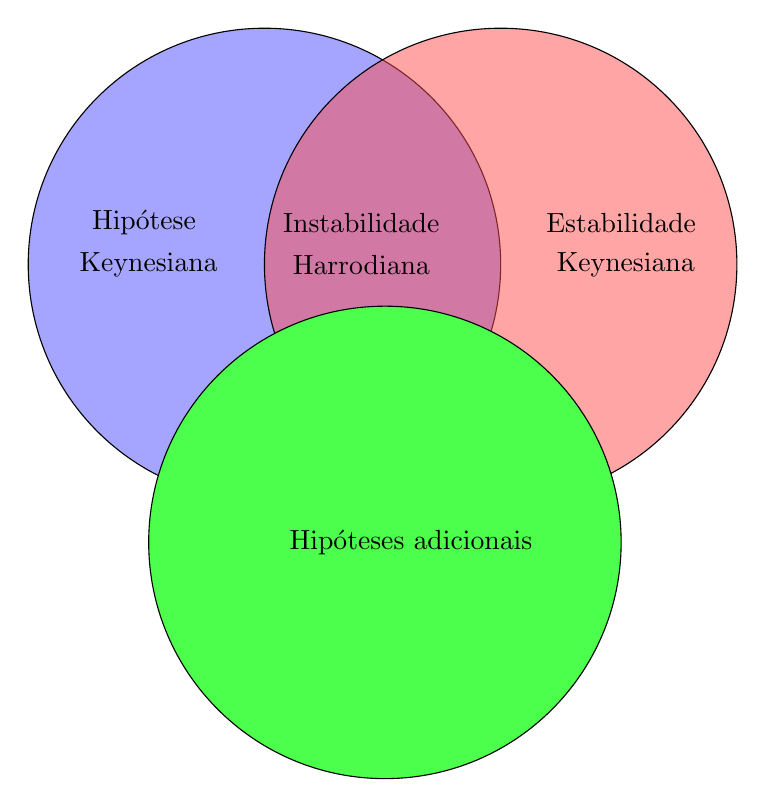
\begin{tikzpicture}
\def\radius{3cm}
\def\mycolorbox#1{\textcolor{#1}{\rule{2ex}{2ex}}}
\colorlet{colori}{blue!70}
\colorlet{colorii}{red!70}
\colorlet{coloriii}{green!70}

\coordinate (ceni);
\coordinate[xshift=\radius] (cenii);
\coordinate[yshift=-3.5\radius, xshift=1.5\radius] (ceniii);

\draw[fill=colori,fill opacity=0.5] (ceni) circle (\radius);
\draw[fill=colorii,fill opacity=0.5] (cenii) circle (\radius);
\draw[fill=coloriii,fill opacity=1] (ceniii) circle (\radius);


\node[yshift=.5\radius, xshift=-1.5\radius] at (ceni) {\text{Hipótese}};
\node[xshift=-1.5\radius] at (ceni) {\text{ Keynesiana}};
\node[yshift=.5\radius, xshift=1.5\radius] at (cenii) {\text{Estabilidade}};
\node[xshift=1.5\radius] at (cenii) {\text{ Keynesiana}};
\node[yshift=.5\radius, xshift=1.2\radius] at (ceni) {\text{Instabilidade}};
\node[xshift=1.2\radius] at (ceni) {\text{Harrodiana}};
\node[xshift=.3\radius] at (ceniii) {\text{Hipóteses adicionais}};
\end{tikzpicture}
\caption*{\textbf{Fonte:} Elaboração própria}
\end{figure}
\end{comment}